\section{\label{sec:LHCb}Trigger system of the LHCb experiment}
%Kaare, Carlos


%\begin{figure}[ht]
%    \centering
%    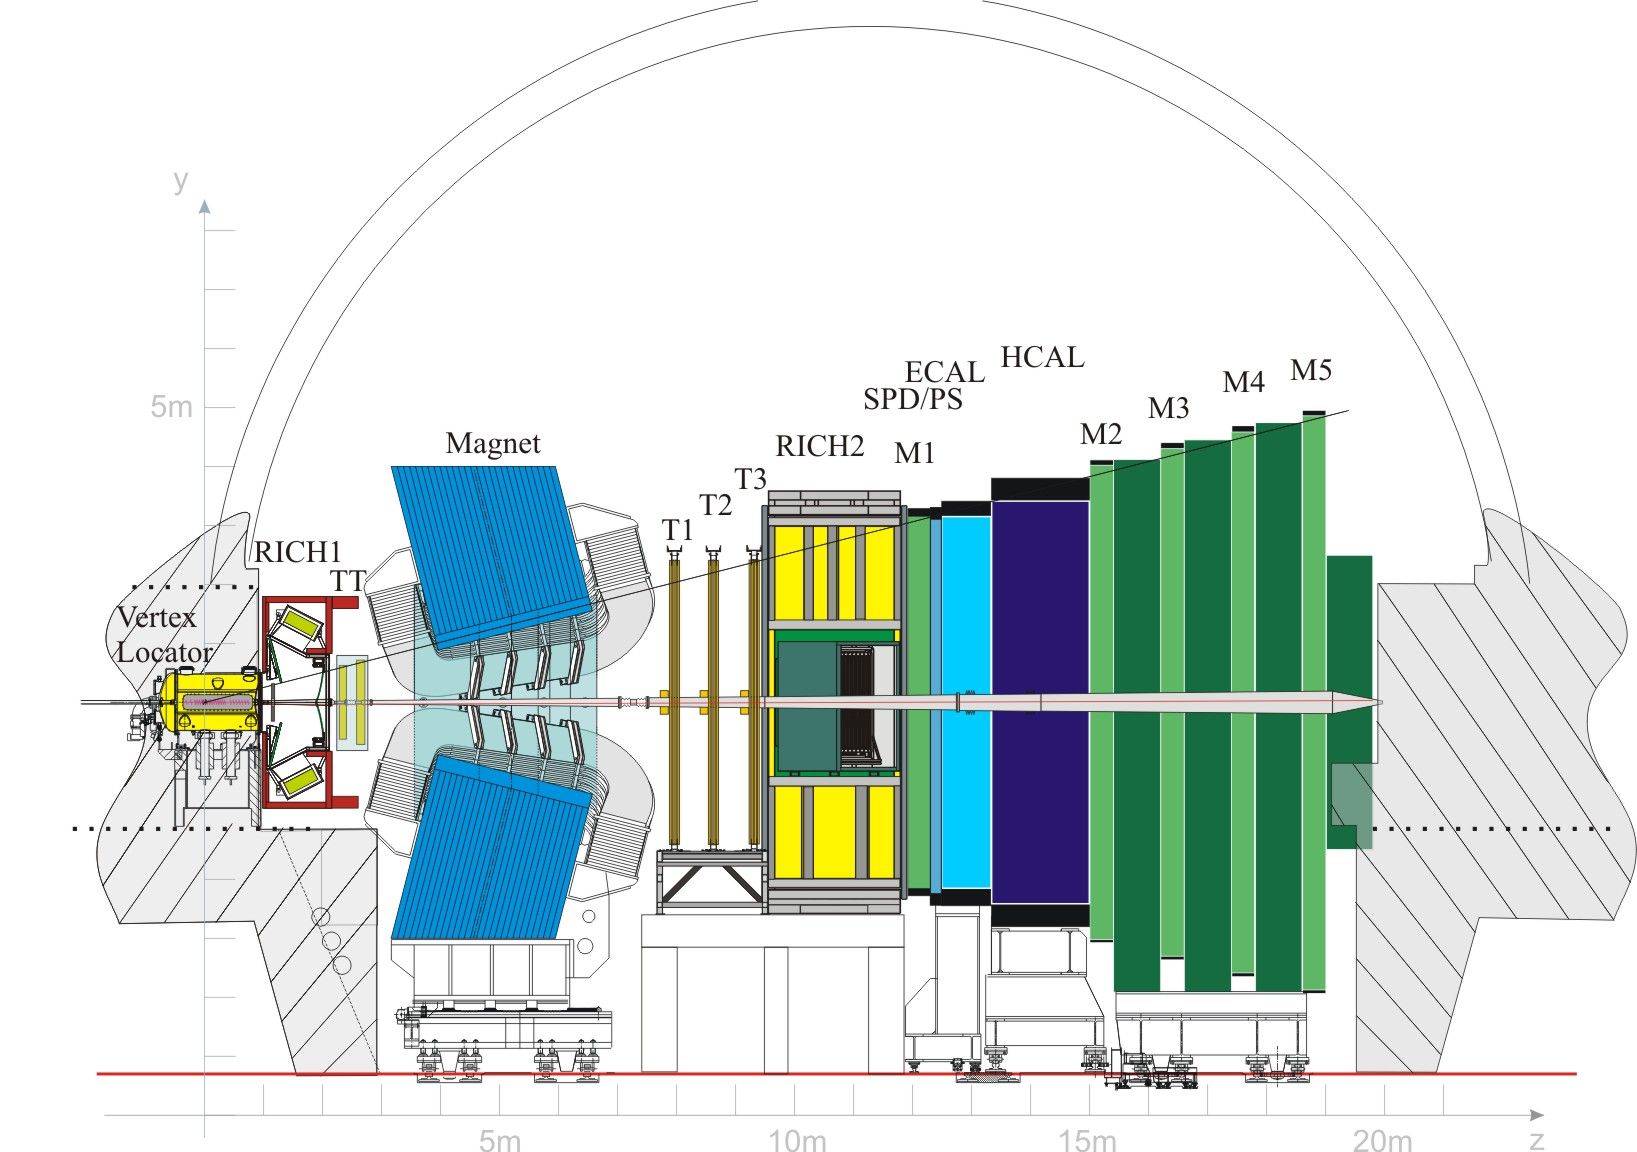
\includegraphics[width=0.7\linewidth]{images/lhcb/Lhcbview.jpg}
%    \caption{A cross section of the upgraded LHCb detector\cite{LHCb_2008}.}
%    \label{lhcb-detector}
%\end{figure}

%\subsection{The LCHb Detector}

%The layout of the upgraded LHCb detector is shown in figure \ref{lhcb-detector}. 
The components of the detector can be categorized into three subsystems: The tracking system, particle identification and data acquisition. For Run~3, the tracking system consists of the vertex locator (VELO), an array of pixel silicon detectors surrounding the interaction region; the upstream tracker (UT), a series of silicon strips preceding the magnet; and the SciFi Tracker system, three scintillating fiber tracker stations located downstream of the LHCb dipole magnet. The particle identification system is comprised of two ring imaging Cherenkov detectors (RICH1 and RICH2), an electromagnetic calorimeter (ECAL), a hadronic calorimeter (HCAL) and four muon chambers (M2–5). The data acquisition covers the front-end electronics (FE) and back-end (BE) electronics, the event-builder and the event-filter farms~\cite{LHCb:2023hlw}.

\subsection{Previous Iterations of the LHCb trigger system}%Kaare


\begin{figure}[h!]
    \centering
    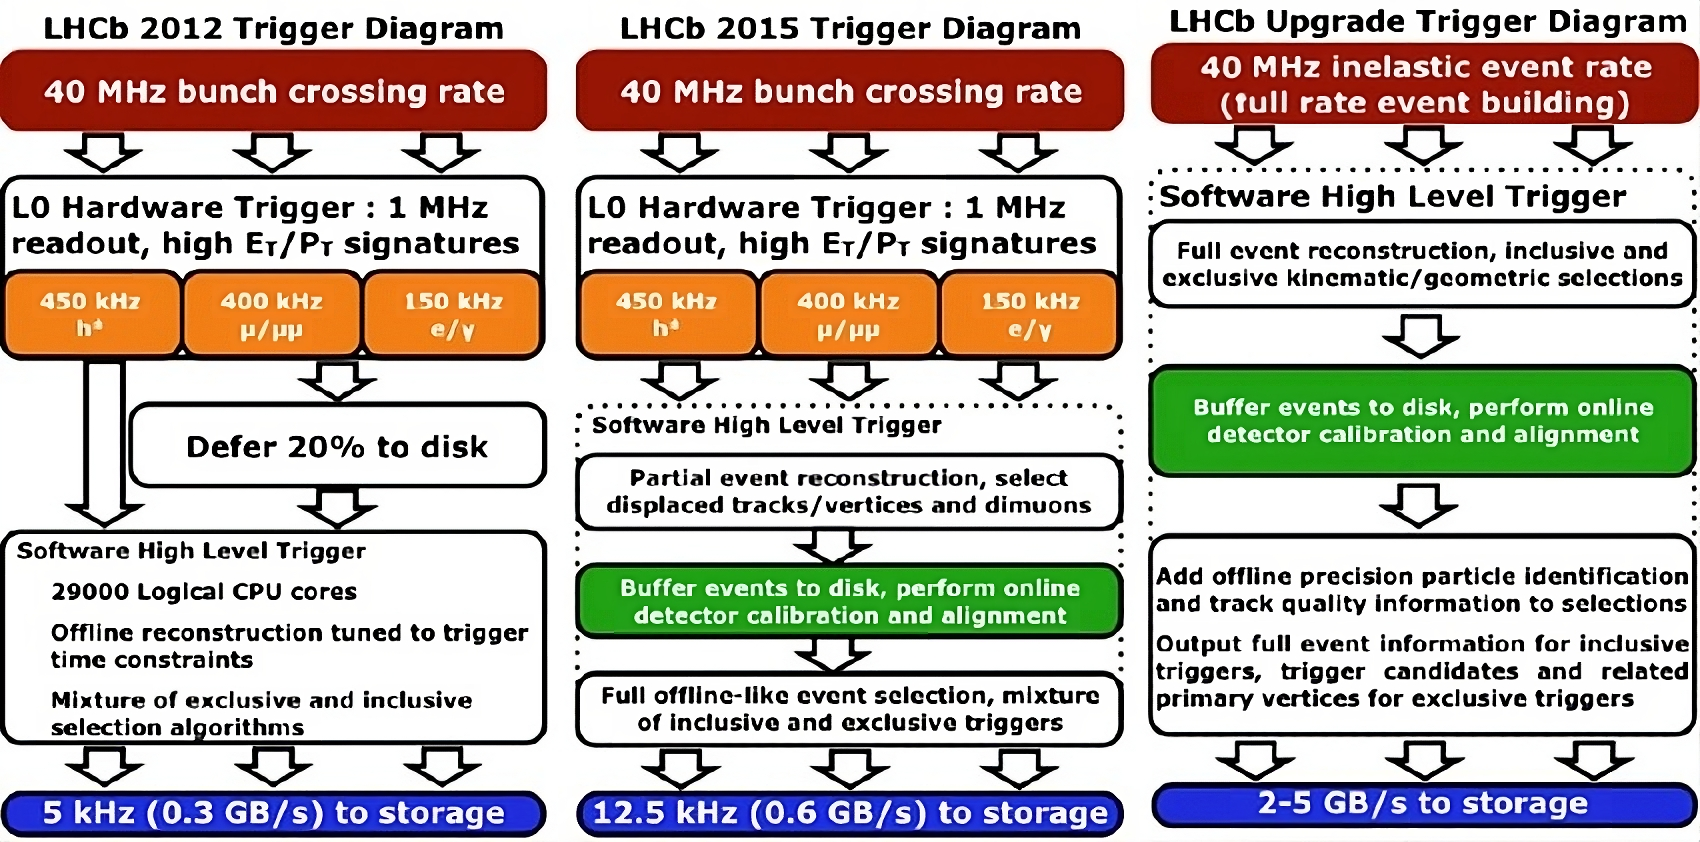
\includegraphics[width=1\linewidth]{images/lhcb/Diagrams-of-the-LHCb-trigger.png}
    \caption{Diagrams of the LHCb trigger data-flow in Run~1 (left), Run~2 (center) and  Run~3 (right) \cite{LHCb_Szumlak_2017}.}
    \label{lhcb-hlt}
\end{figure}

Figure \ref{lhcb-hlt} shows diagrams of the LHCb triggers for Run~1, Run~2 and Run~3, from left to right. %The three different iterations of the trigger system will be covered in the following sections.
For Run~1, the LHCb trigger system consisted of a hardware trigger (L0) and a software trigger. The main goal of the hardware trigger was to select particles with high transverse energy and transverse momentum using partial detector readout to reduce the event rate from 10 MHz to 1.1~MHz, for which the full detector could be read out. The software high-level trigger ran on 16000 CPU cores on an Event Filter Farm (EFF) and filters events in a two-step process. The first step would confirm the hardware trigger decision by performing a partial event reconstruction. The second step would perform a full reconstruction of events that passed the first step, saving the output to permanent storage at a rate of 5 kHz~\cite{LHCb:Head_2014, LHCb:Albrecht_2014}.



\subsection{Upgraded LHCb trigger system} %\cite{LHCb_upgrade_trigger_TDR removal of hardware trigger \& using GPUs, Allen project }%\cite{LHCb_Allen_GPU
%Kaare


The current LHCb trigger system is the result of the upgrades made preceding Run~3. The full resulting trigger dataflow is shown in Figure \ref{lhcb-hlt-run-III}.

\begin{figure}[ht]
    \centering
    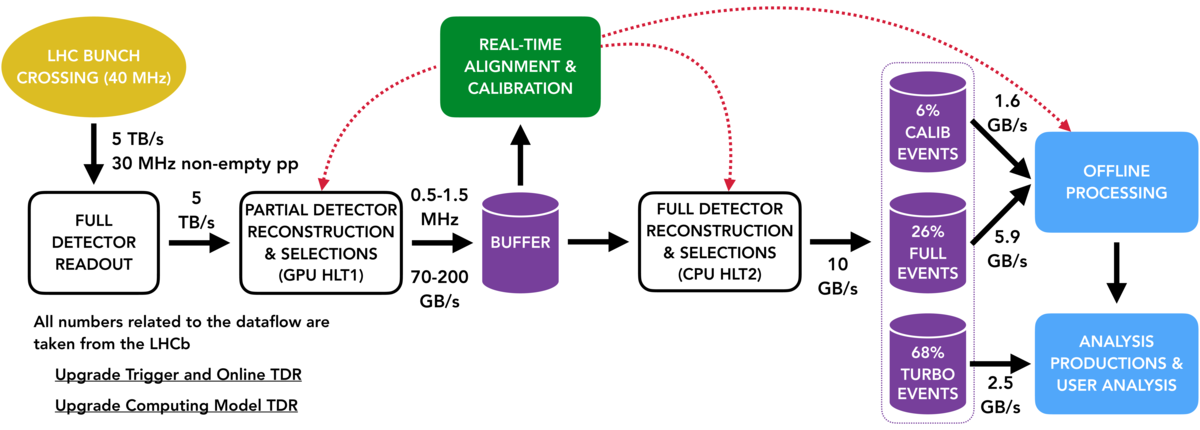
\includegraphics[width=1\linewidth]{images/lhcb/hidef_RTA_dataflow_widescreen.png}
    \caption{Diagram of the LHCb Run~3 trigger~\cite{run3-dataflow}.}
    \label{lhcb-hlt-run-III}
\end{figure}


\subsubsection{GPU HLT1}



\subsubsection{CPU HLT2}

The most useful type of track is the ``Long track", which has hits in the VELO and the SciFi and can also have hits in the UT. The main task of HLT2 is to identify these long tracks, and in Run III, this is done using the Matching and Forward Tracking algorithms. The Matching algorithm takes as input ``VELO tracks" from the VELO (reconstructed using the VELO Tracking algorithm~\cite{LHCb_VELO_tracker}) and ``T tracks" from the SciFi (reconstructed using the Hybrid Seeding algorithm~\cite{LHCb_HybridSeeding}) and matches them, making them Long tracks. The Forward Tracking algorithm then tries to match unmatched VELO tracks with SciFi hits that are not already part of a Long track~\cite{LHCb_HLT2}. 

The HLT2 classification outputs the events, at a rate of 10 Gb/s, in a custom format called Turbo Stream that preserves only the candidates reconstructed by the trigger discarding the rest of the event, thus reducing the event size of an order of magnitude to finally write on tape.


\subsection{The Turbo persistence model} %\cite{LHCb:2018zdd,Aaij:2016rxn,Aaij:2019uij}
%CARLOS


 
%\begin{figure}[h!]
%    \centering
%    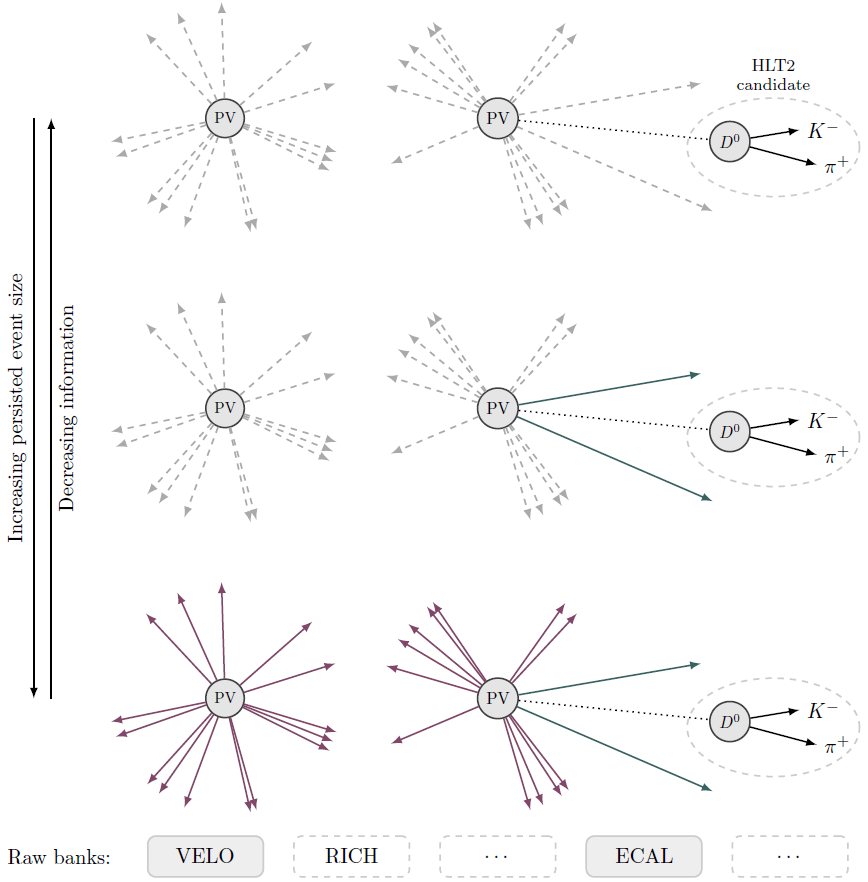
\includegraphics[width=0.7\linewidth]{images/lhcb%/persistency.png}
%    \caption{A visualisation of the same reconstructed event with varying levels of object persistence:
%Turbo (top); selective persistence (middle); and complete reconstruction persistence (bottom).
%Solid objects are those persisted in each case. A trigger selection may also ask for one or more sub-detector raw banks to also be stored, shown as solid rectangles.}
%    \label{lhcb-persistency}
%\end{figure}


\subsection {Real-time alignment and calibration in Run 2 \& Run 3}%\cite{Aaij:2019uij,Borghi:2017hfp,Reiss:2846414}
%CARLOS



